\section{Converged Graph Relational Optimization Framework}

In this section, we first introduce the sketch of the converged graph relational optimizer.
Then, Section \ref{sec:framework:combination} presents the workflow of the framework, and Section \ref{sec:framework:detailed-optimizations} explains the optimization strategies applied in the framework in detail.

\begin{figure}
    \centering
    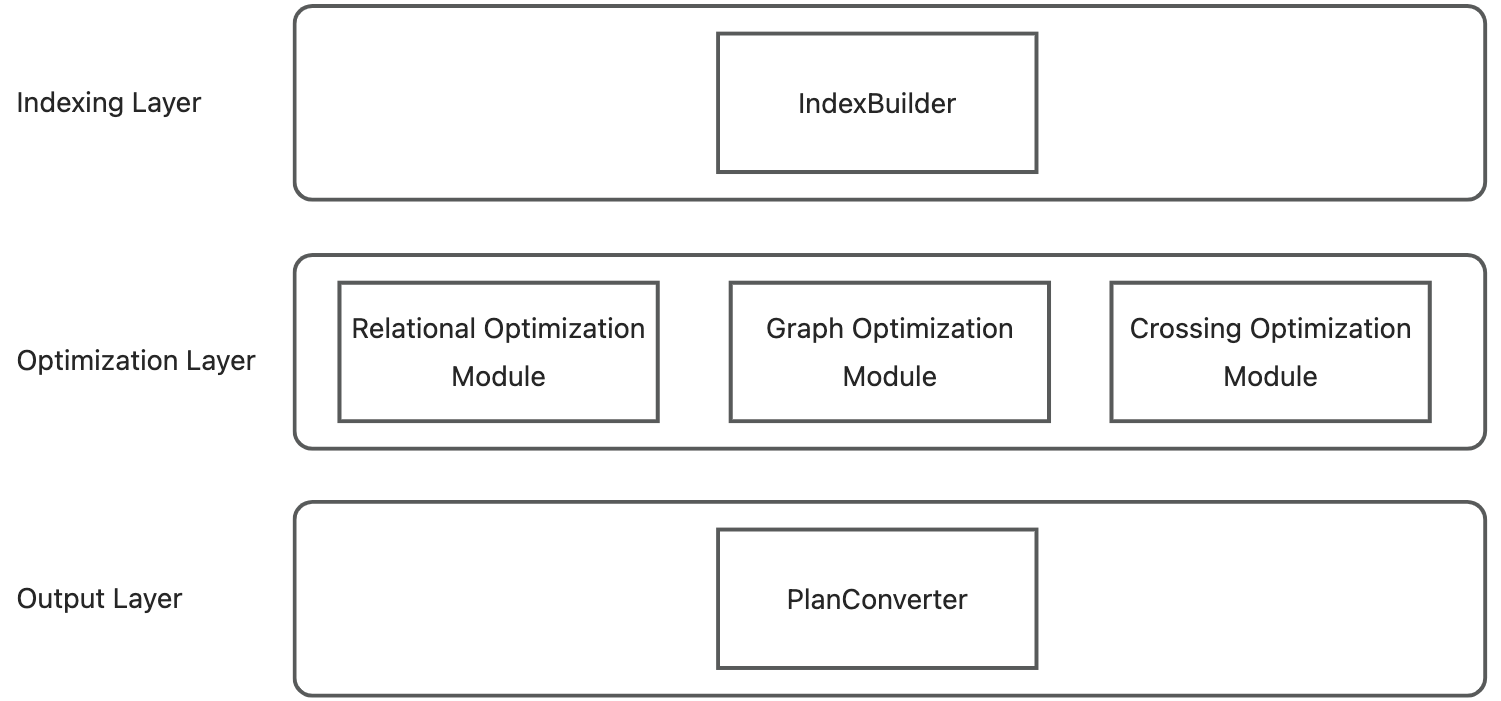
\includegraphics[width=\linewidth]{./figures/framework.png}
    \caption{Overview of the Converged Graph Relational Optimization Framwork.}
    \label{fig:framework-overview}
\end{figure}

\subsection{Overview of the Framework}

% A system overview figure and some introduction
The framework consists of three layers as shown in Fig.~\ref{fig:framework-overview}, i.e., indexing layer, optimization layer, and output layer.
In this subsection, the details of these three layers are introduced in detail.

\textbf{Indexing Layer.} The indexing layer mainly builds graph indices for the graph optimization module with IndexBuilder.
For the graph queries specified in the SQL/PGQ query, the obtained graph plans are likely to contain the commonly used graph operators (e.g., \textit{GetVertex}, \textit{GetEdge}, and \textit{GetNeighbor}).
However, traditional relational databases cannot support such operators efficiently.
Therefore, graph indices need to be constructed so that vertices can efficiently access its adjacent edges and neighboring vertices, and edges can also quickly obtain their adjacent vertices.
Then, in the process of optimizing the graph subplans, the cost of graph operators like \textit{GetNeighbor} should be that of obtaining neighbors of vertices in relational databases with graph indices.

\textbf{Optimization Layer.} The optimization layer consists of three modules, i.e., the relational optimization module, graph optimization module, and crossing optimization module.
In detail, the relational optimization module optimizes relational queries with relational optimization strategies.
It should contain rule-based optimizations (abbr.~RBOs) and cost-based optimizations (abbr.~CBOs), and can be any one of the commonly used relational optimizers (e.g., Calcite or the optimizer of Duckdb).
The graph optimization module optimizes graph queries and also has specific RBOs and CBOs for graphs queries.
It can be any existing graph optimizer (e.g., GLogue).
Besides, the crossing optimization module optimizes the relational queries and graph queries simultaneously.
Optimizations are achieved through interaction and transformation between relational and graph queries.

\textbf{Output Layer.} The output layer converts the execution plan obtained in the optimization layer to the plan that can be executed by the target database.
To ensure the flexibility of the framework, codegen technology is utilized to implement the PlanConverter.
In detail, the PlanConverter first converts the obtained execution plan into the predefined internal representation, and then the internal representation is transformed into a physical plan that the target database can parse and execute.

\begin{figure}
    \centering
    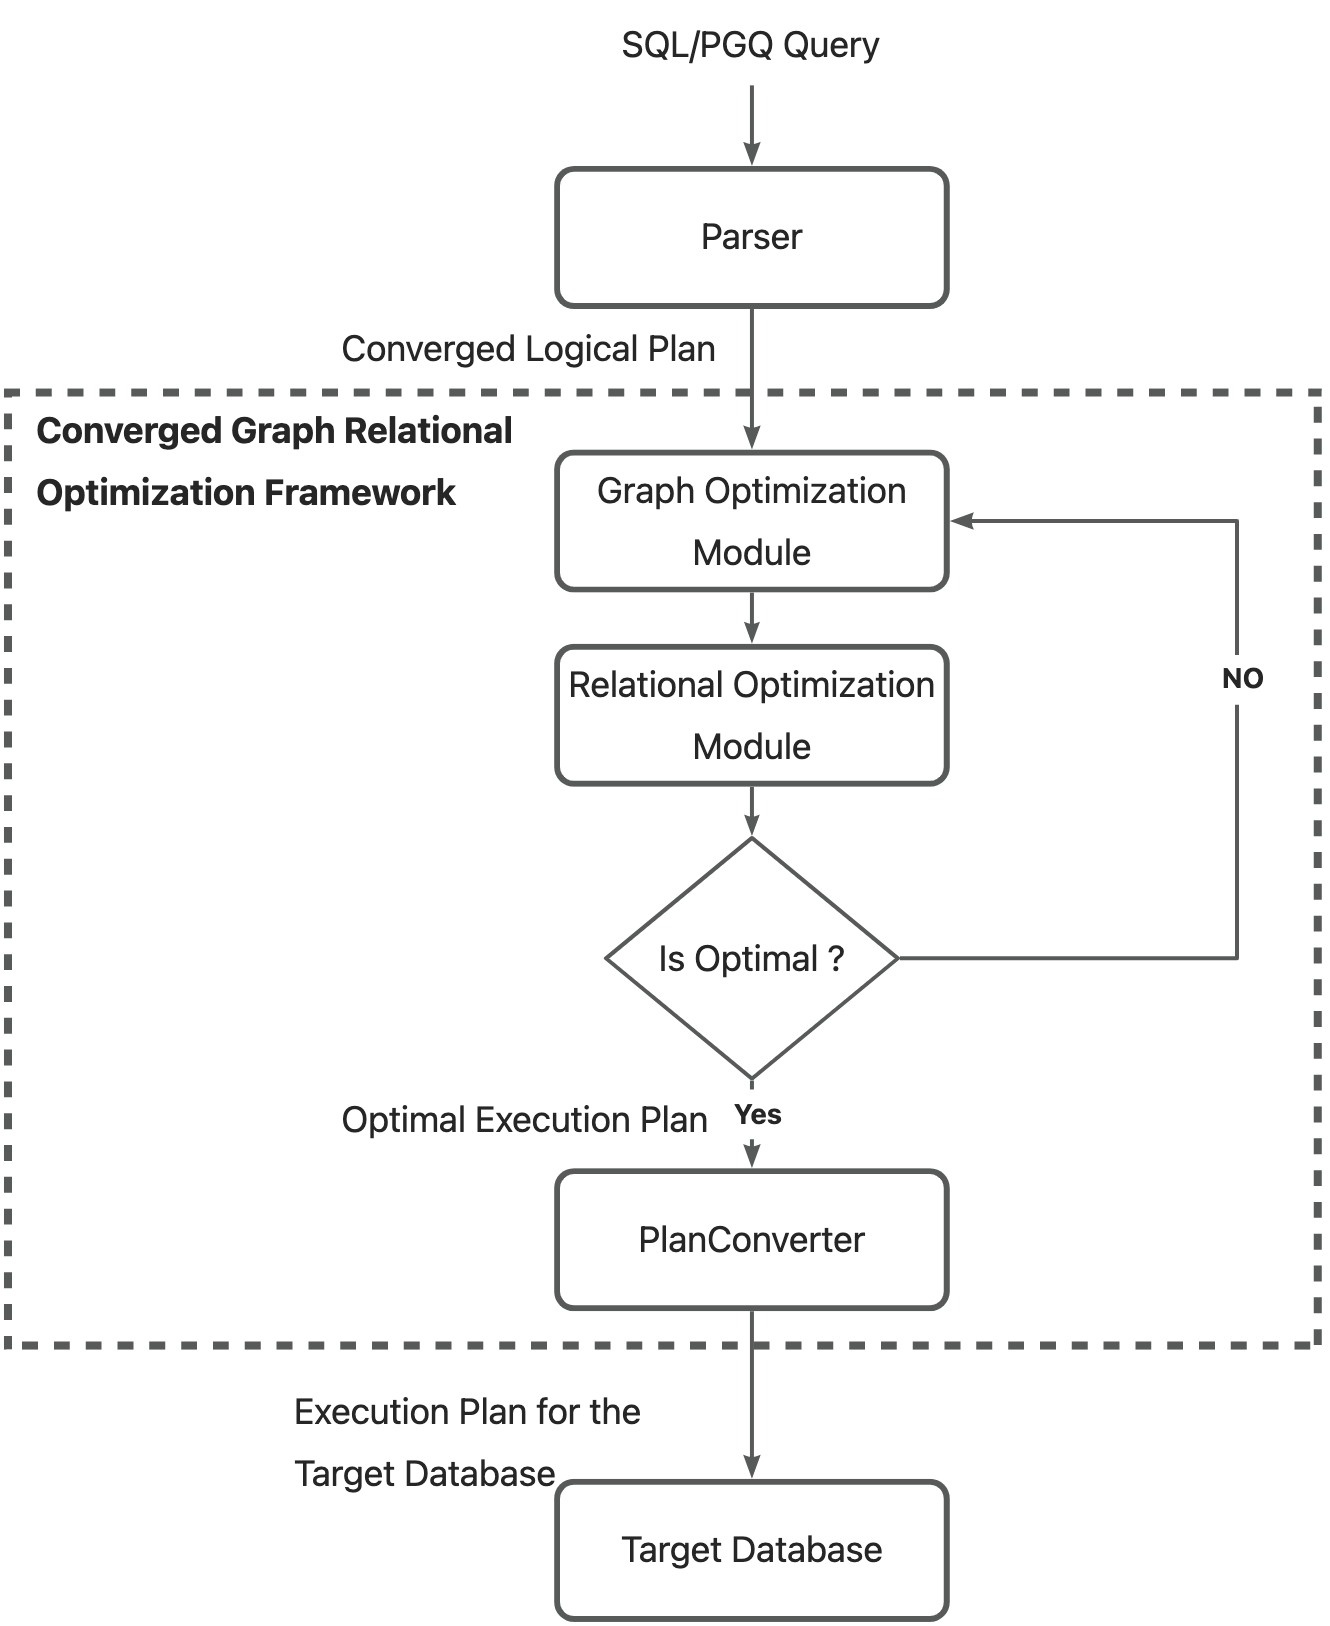
\includegraphics[width=\linewidth]{./figures/workflow.png}
    \caption{Workflow of the Converged Graph Relational Optimization Framework.}
    \label{fig:workflow}
\end{figure}

\subsection{Leveraging Benefits of Both Relational and Graph Optimizations}
\label{sec:framework:combination}

\begin{figure*}
    \centering
    \begin{subfigure}[b]{0.4\linewidth}
        \centering
        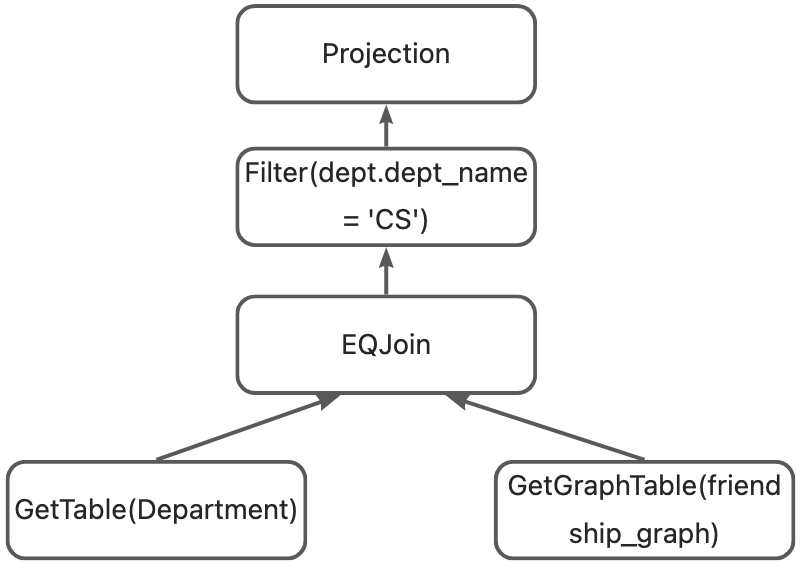
\includegraphics[width=\linewidth]{./figures/converged-logical-plan-relational.png}
        \caption{Relational Subplan of the Converged Logical Plan.}
        \label{fig:converged-logical-plan-relational}
    \end{subfigure}
    \begin{subfigure}[b]{0.4\linewidth}
        \centering
        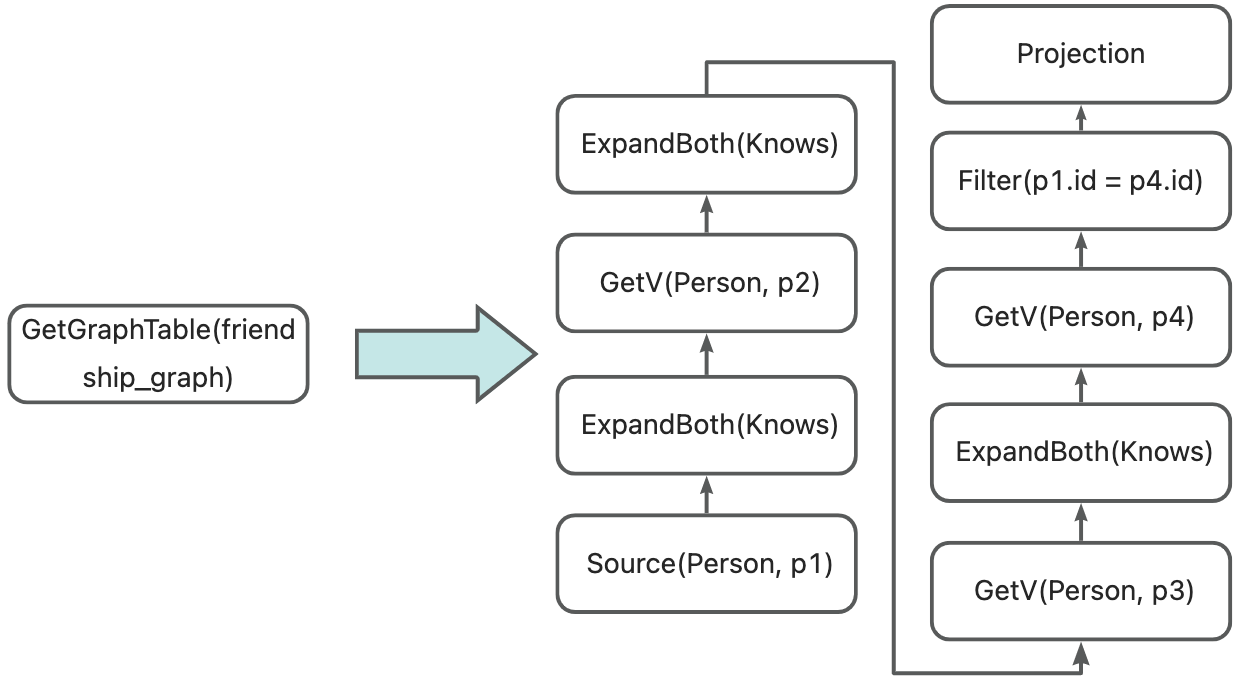
\includegraphics[width=\linewidth]{./figures/converged-logical-plan-graph.png}
        \caption{Graph Subplan of the Converged Logical Plan.}
        \label{fig:converged-logical-plan-graph}
    \end{subfigure}
    \begin{subfigure}[b]{0.4\linewidth}
        \centering
        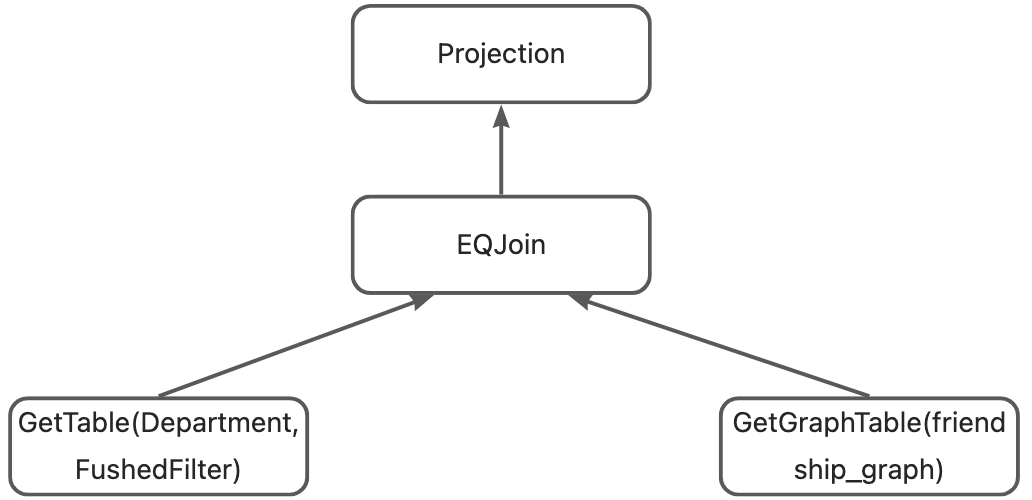
\includegraphics[width=\linewidth]{./figures/converged-logical-plan-relational-optimized.png}
        \caption{Relational Subplan after Optimization.}
        \label{fig:relational-plan-optimized}
    \end{subfigure}
    \begin{subfigure}[b]{0.4\linewidth}
        \centering
        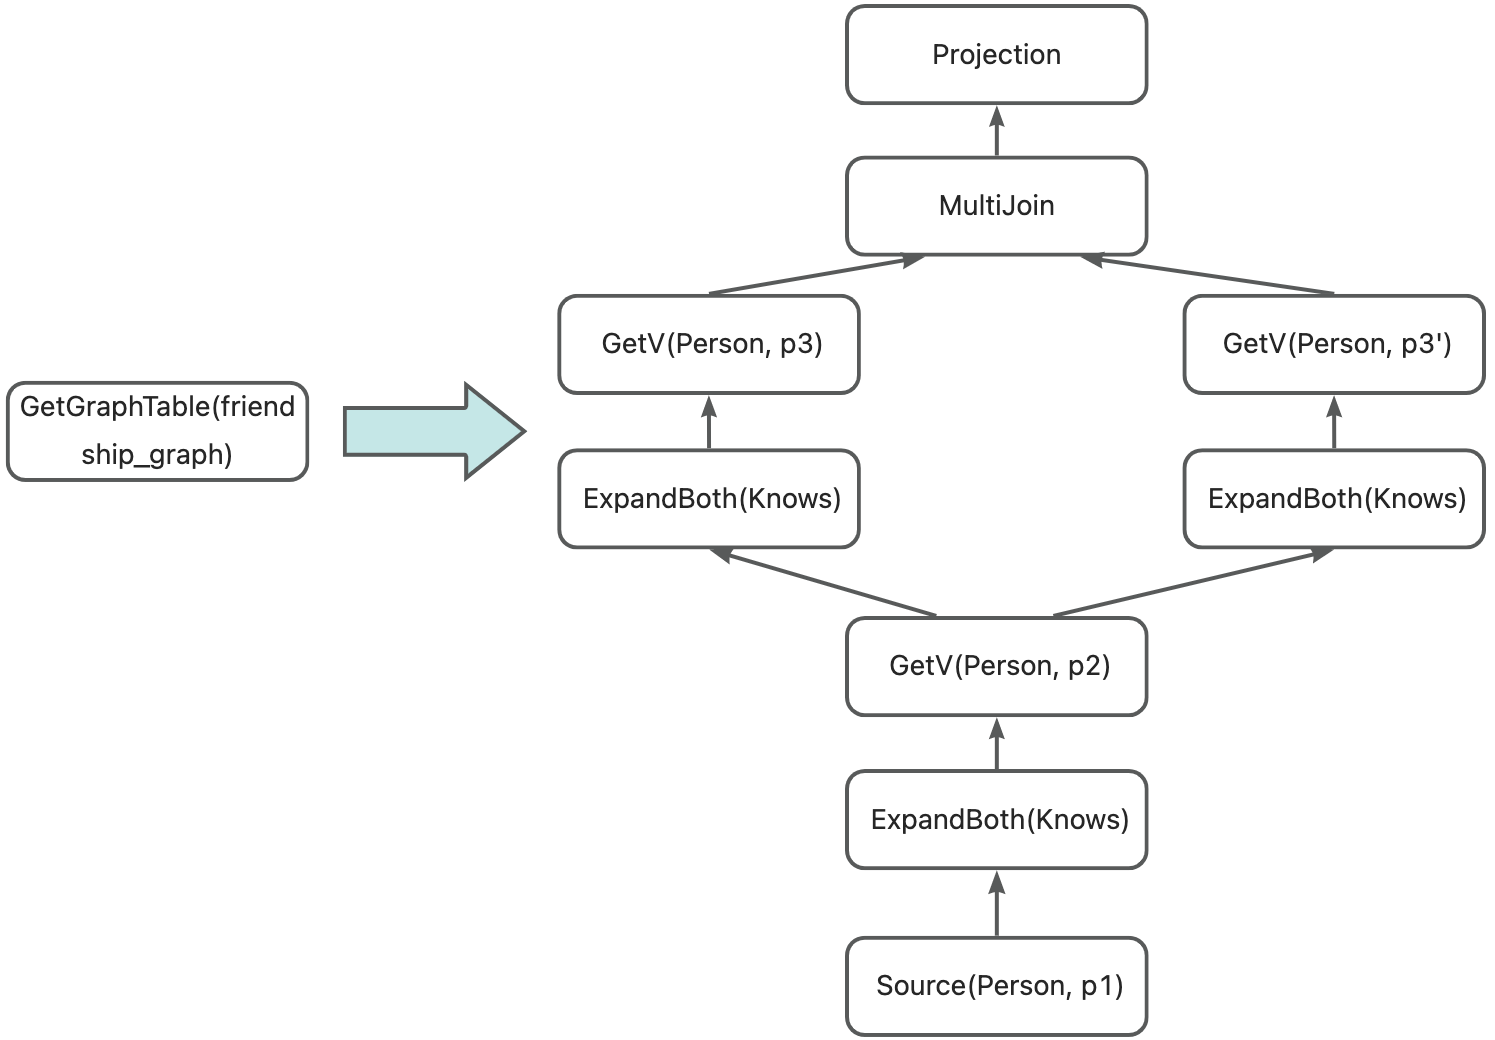
\includegraphics[width=\linewidth]{./figures/converged-logical-plan-graph-optimized.png}
        \caption{Graph Subplan after Optimization.}
        \label{fig:graph-plan-optimized}
    \end{subfigure}
    \begin{subfigure}[b]{0.4\linewidth}
        \centering
        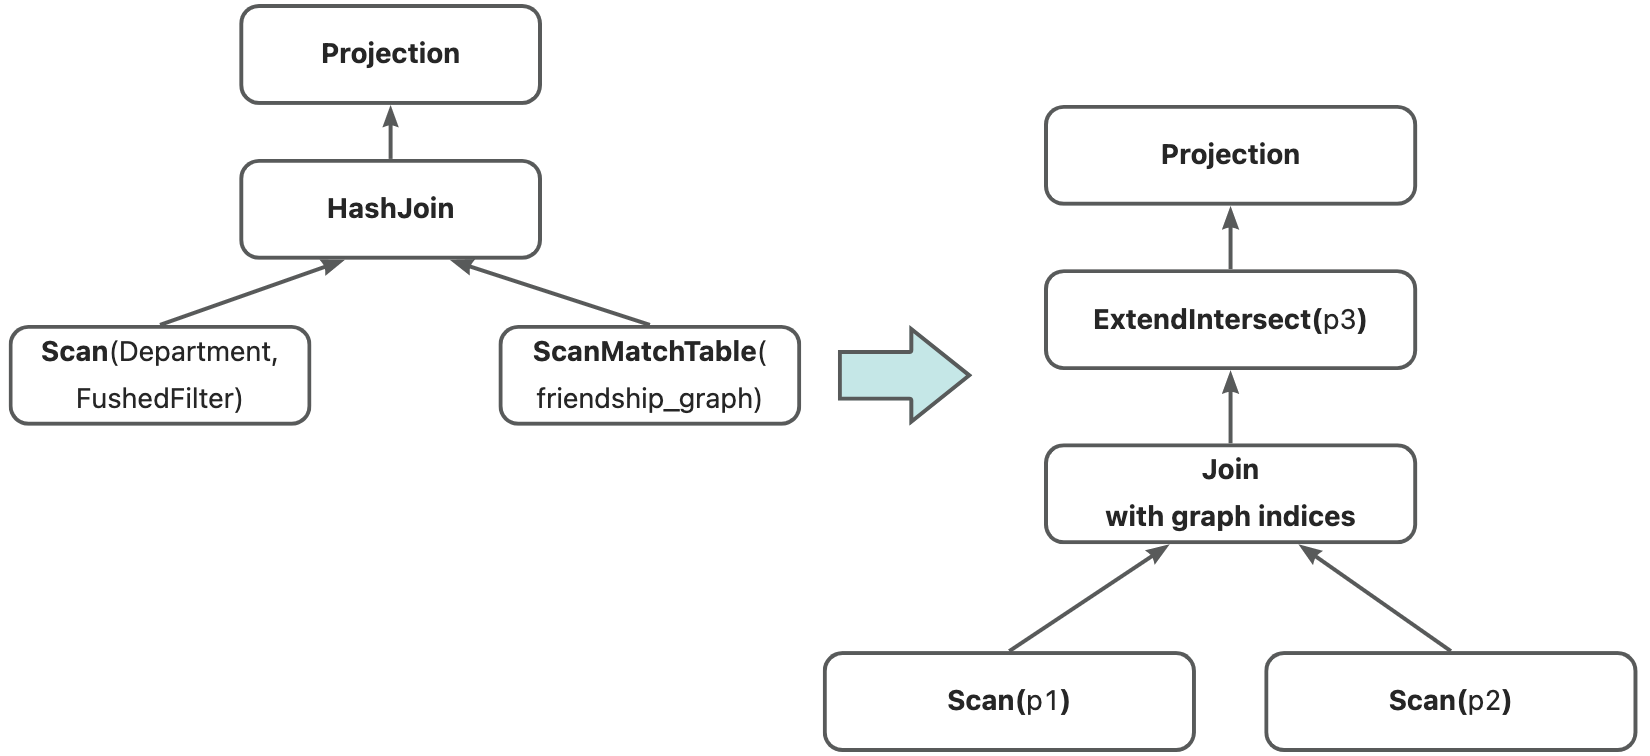
\includegraphics[width=\linewidth]{./figures/converged-physical-plan.png}
        \caption{Obtained Optimial Physical Plan.}
        \label{fig:physical-plan-optimized}
    \end{subfigure}
    \caption{An example of query opitmization.}
    \label{fig:query-grtree-example}
\end{figure*}


Fig.~\ref{fig:workflow} illustrates the workflow for optimizing a query that adheres to the SQL/PGQ grammar using the converged graph relational optimization framework.
In detail, the query is first parsed and a converged logical plan is generated.
The converged logical plan consists of several graph subplans and a relational subplan.
Eacn graph subplan corresponds to a graph query, and it is optimized with the graph optimization module.
Since parts of the graph query are always marked with ``GRAPH\_TABLE (name, MATCH $\cdots$)'', it is straightforward to distinguish graph queries from relational queries, and the graph subplans can be generated easily.
For each graph subplan, an operator ``GetGraphTable(name)'' is generated and added to the relational subplan.
Specifically, from the perspective of the relational optimization module, the ``GetGraphTable'' operator is simply an operator for retrieving data like ``GetTable'' and it returns table data.
Please note that since the outputs of graph queries need to be relational tables as defined in SQL/PGQ, a graph query can be utilized as a subquery to retrieve the table involved in the relational query.
However, a relational query cannot serve as a subquery within a graph query because the mappings between relational tables and vertices/edges need to be specified beforehand, and the graph indices should be built in advance.


With the generated converged logical plan, the converged optimizer takes effect and obtains the optimal physical plan with the modules in the optimization layer.
Specifically, the crossing optimization module first takes effects, e.g., pushing filtering conditions from the relational subquery to graph subqueries.
Then, the graph subqueries are optimized with the graph optimization module.
During the process of optimizing the graph subqueries, the cardinalities of the outputs of the graph subqueries are also estimated.
Next, the relational optimization module is utilized to optimize the relational query, where some source tables may be the outputs of graph subqueries.
After that, it is tested whether the crossing optimization module can further optimize the plan.
If the plan can still be optimized, then the three modules are applied again to optimize the plan.
Otherwise, the optimal execution plan is obtained.

After the optimal physical plan is obtained, the PlanConverter transforms the plan to an internal representation (e.g., substrait), and then the internal representation is transformed to the physical plan that can be executed by the target database.
Finally, the plan is executed and the query results are obtained.
The above process of query processing is illustrated with the following example.

\begin{example}
    Given a relational database with tables as follows,
    \begin{equation*}
        \begin{split}
            & \textit{Person = (\underline{id}, name, dept\_id)} \\
            & \textit{Knows = (\underline{id1}, \underline{id2})} \\
            & \textit{Department = (\underline{dept\_id}, dept\_name)}, \\
        \end{split}
    \end{equation*}
    suppose we are going to find three persons satisfying: 
    (1) These three persons know each other;
    (2) At least two of them are from the department of computer science.
    The SQL/PGQ query for this task is shown in Example \ref{example:introduction:sqlpgq}.      

    There is one graph query for obtaining triangles of persons that know each other.
    Therefore, the converged logical plan consists of one relational subplan and one graph subplan.
    The algebra expression corresponding to this query is as follows:
    Firstly, to obtain the triangles, the graph relational algebra expression is
    \begin{equation*}
        \begin{split}
            G_{\triangle} = & \sigma_{p4.id = p1.id}(\updownarrow_{(p3)}^{(p4)}[:Knows]\updownarrow_{(p2)}^{(p3:Person)}[:Knows] \\
            & \updownarrow_{(p1)}^{(p2:Person)}[:Knows]\bigcirc_{(p1:Person)}).
        \end{split}
    \end{equation*}
    Then, to get the results of the graph query and formulate the results as a relational table, the algebra expression is 
    \begin{equation*}
        \begin{split}
            R_{graph} = & \pi_{p1.name\rightarrow pn1, p1.dept\_id \rightarrow dept1,p2.name\rightarrow pn2, p2.dept\_id \rightarrow dept2,} \\
            & _{p3.name\rightarrow pn3, p3.dept\_id \rightarrow dept3}(G_{\triangle}).
        \end{split}
    \end{equation*}
    Finally, to obtain the triangles of persons with at least two persons from the department of computer science, the relational algebra expression is
    \begin{equation*}
        \begin{split}
        \pi_{pn1, pn2, pn3}
        (& \sigma_{dept.dept\_name = `Computer Science'}( \\ 
        & dept \Join_{dept1=dept.dept\_id \land dept2=dept.dept\_id} R_{graph})).
        \end{split}
    \end{equation*}

    Based on the above algebra expressions, the corresponding converged logical plan is shown, and its relational and graph subplans are presented in Fig.~\ref{fig:converged-logical-plan-relational} and Fig.~\ref{fig:converged-logical-plan-graph}, repsectively.
    
    Then, optimization modules in the optimization layer are applied to optimize the relational subplan and graph subplans.
    The optimized converged logical plan is shown in Fig.~\ref{fig:relational-plan-optimized} and Fig.~\ref{fig:graph-plan-optimized}.
    Moreover, the finally obtained optimal physical plan is shown in Fig.~\ref{fig:physical-plan-optimized}.
\end{example}

\subsection{Detailed Optimizations}
\label{sec:framework:detailed-optimizations}

In this subsection, we first present the optimization strategies utilized in the relational optimization module and graph optimization module, respectively.
Then, the strategies of crossing optimization module are also proposed.

\subsubsection{Optimization Strategies in Relational Optimization Module}

Like most relational optimizers, the relational optimization module applies both Rule-based Optimization (abbr.~RBO) and Cost-based Optimization (abbr.~CBO) strategies on relational subplans for a better physical plan.
In detail, in terms of RBO, commonly used optimizations such as filter pushdown, join order optimization, and removal of unused columns are employed in the converged optimizer.
In terms of CBO, the costs of plans are estimated based on the low-order statistics such as the cardinalities of tables and query conditions.



\subsubsection{Optimization Strategies in Graph Optimization Module}

In the graph optimization module, we formulate a specific rule set to capitalize on optimization potential among graph operators. 
Both RBO and CBO strategies are included in the rule set.

In terms of RBO strategies, two frequently utilized key rules, i.e., \trimrule and \fusionrule, are presented in this subsection.

\trimrule. 
The \trimrule~ is a well-established relational optimization strategy that removes superfluous data at intermediary stages of query processing. 
Two particular instances where trimming helps include: 
Firstly, \trimrule~ can eliminate intermediate results with aliases that are not required and reduce computations.
Secondly, it involves discarding unneeded vertex and edge properties when retrieving from the data graph. 
This is accomplished by specifying essential properties in the graph operators’ \code{COLUMNS} field.
Formally, an example of applying \trimrule is as follows:
\begin{equation}
    \mathcal{S}_g \Rightarrow \pi_{u.a_1, \cdots, u.a_k}\mathcal{S} _g 
\end{equation}
where $\mathcal{P}_g$ is a graph relational algebra expression corresponding to a graph subplan, and $u.a_1, \cdots, u.a_k$ are necessary properties.


\fusionrule. 
The \fusionrule~ is a graph-centric rule. 
Commonly in graph queries, a sequence of \expandedge~ followed by \getvertex~ indicates a search for neighboring vertices. 
The \fusionrule~ consolidates these operators into one integrated \expandvertex~ to boost efficiency. 
Nonetheless, whether \expandedge~ and \getvertex~ can be merged is context-dependent. 
For example, if some properties of the edges are needed, fusion might not be feasible.
This rule evaluates such factors to ensure query optimization without compromising result integrity.
%Formally, an example of applying \fusionrule is as follows:
%\begin{equation}
%    \begin{split}
%    &  \\
%    & \hspace*{2em} \Rightarrow \pi_{u.a_1, \cdots, u.a_k}\updownarrow_{(u)}^{(v:vLabel)}[:eLabel](\sigma_{d(u)}\bigcirc_{(u:uLabel)}), \\
%    \end{split}
%\end{equation}
%where $d(u)$ is a filtering constraint on vertex $u$.


In terms of CBO, drawing from insignts gained in the prior research, we implement effective pattern matching by incorporating hybrid pattern join strategies and leveraging high-order statistics, which provide a more granular understanding of the data through the frequency of smaller patterns.
Moreover, the prior research has some drawbacks, including using a bottom-up search framework that potentially missed early pruning opportunities and having a narrow focus on basic patterns without accommodating union patterns scenarios.
Therefore, we also introduce a novel top-down search framework, inclusive of branch-and-bound pruning strategies, and devise specific cardinality estimation methods for union patterns. 
Besides, in this implementation, we use a rule for pattern transformation to ensure all modifications maintain the original results’ integrity.
Furthermore, for pattern matching, we consider binary join and extend-intersect operators. 
The binary join applies a hash-join on two pattern mappings to produce a larger pattern's results.
The extend-intersect operator optimizes the process when only one vertex is added to the existing pattern. 
This expansion can vary from a simple addition of a single new edge to more complex scenarios involving multiple edges, implemented through optimal joins.

Regarding cost and cardinality estimation, we adopt a cost model that considers both the communication costs of intermediate result transfer in distributed environments and the computational costs of physical plan operators. 
Specifically, costs for the binary join and extend-intersect operators in graphs are defined. 
Additionally, we estimate the operator cost using an expand ratio that reflects the change in pattern occurrences when edges are expanded.

\subsubsection{Optimization Strategies in Crossing Optimization Module}

Please note that the optimizations of graph subplans and the relational subplan are not isolated or entirely unconnected.
For example, when \trimrule~ is applied on graph subplans, it is necessary to judge whether the properties of vertices and edges are utilized in graph subplans and relational subplans.
Actually, more crossing optimization strategies can be designed for optimizing the graph and relational subplans simultaneously.
Such optimizations are included in the crossing optimization module, and two typical and crucial strategies of them are \filterrule and \intersectrule. 

\filterrule. 
The \filterrule seeks to push filtering conditions on properties of graph elements from the relational subplan to graph subplans, so that invalid graph elements can be dropped earlier.
An example of applying \filterrule is given in Example \ref{example:push_down}.

Specifically, \filterrule can embed filtering conditions into basic graph operators like \scan~, \expandedge~, or \getvertex~ to further push down filtering conditions in graph queries. 
This integration allows the direct exclusion of vertices and edges not satisfying the filter conditions, thus drastically cutting down the volume of intermediary outcomes.

Formally, the equation rule w.r.t.~\filterrule is as follows:
\begin{equation}
    \begin{split}
    & \sigma_{\theta}\pi_{v.a_1, \cdots, v.a_k}(lr~\alpha_{(u)}^{(v)}[e]~er) \\
    & \hspace*{2em} \equiv \pi_{v.a_1, \cdots, v.a_k}(lr~\sigma_{\theta}(\alpha_{(u)}^{(v:vLabel)}[e]~er)), \\
    \end{split}
\end{equation}
where $lr$ and $er$ are graph relational algebra expressions, $\alpha \in \{\uparrow, \downarrow, \updownarrow\}$, and vLabel is specified if the label of $v$ is specified in $\theta$.


\intersectrule. 
Please note that the intersection operator is not defined in graph queries, but it can be expressed with expand operators.
Given a SQL/PGQ query, if the two subqueries that intersect are both graph queries, then the paths in these two graph queries can be combined with expand operators to generate new paths.
That is, two graph queries combined with an intersection operator is converted to a new graph query.
By leveraging graph indices, it can be more efficient to obtain the intersection results w.r.t.~the new graph query.
The rule is as follows.
\begin{equation}
    \begin{split}
        & \pi_{u.a_1, \cdots, u.a_k}(el~\alpha_{(u)}^{v:vlabel}[e]~er) \\
        & \hspace*{2em} \equiv \pi_{u.a_1, \cdots, u.a_k}(el) \cap \pi_{u.a_1, \cdots, u.a_k}(\alpha_{(u)}^{v:vlabel}[e]~er),
    \end{split}
\end{equation}
where $el$ and $er$ are graph relational algebra expressions, $\alpha \in \{\uparrow, \downarrow, \updownarrow\}$.